%===================================== CHAP 5 =================================


\chapter{Solution Framework} \label{chapter_solution_approach}

The FPLDP is a complex problem with a high degree of uncertainty. In each gameweek, a broad range of decisions must be optimized. Compared to other Fantasy Sports, the gamechips make it even more complicated. If the model presented in Chapter \ref{mathematical_model} is run ex-post, it yields the optimal solution as the realized points are known. However, in order to compete in FPL, decisions must be made ex-ante. Thus, estimations of expected points and strategies for when the gamechips should be played are required. The aim of this chapter is to propose a solution framework designed to maximize performance over the entire season. By a framework, a methodology for competing in the FPL on the same terms as managers are meant. Thus, the framework includes a solution method for the mathematical model, a method for generating forecasts of player points and strategies for the use of gamechips. In addition, an approach to handle variance in, and correlation between, player points is included in the framework. This procedure is hereby referred to as risk handling.

\newpar

As seen throughout this chapter, the framework is intended to be solely data-driven. That is, a participant in the FPL applying the framework does not have to make any decision based on his or her own judgment. Thus, the inherent skill and knowledge of the FPL possessed by a participant applying the framework are essentially irrelevant for its performance.

\newpar

In Section \ref{section_solution_method}, a solution method suggested for solving the mathematical model is presented. In Section \ref{Player_Performance}, three different methods for forecasting player performance are described. Finally, in the Sections \ref{Ch.5_Game_chips} and \ref{Ch.5_Variance_tradeoff}, respectively, methods for implementing gamechips and handling risk are proposed.

\newpage 

\section{Solution Method}\label{section_solution_method}

As stochastic programming models seek to leverage probability distribution of uncertain parameters, they are regarded as more computationally demanding than deterministic programming models \citep{Shapiro}. A conventional method for solving a stochastic model is by use of scenario generation. For the FPLDP, the number of scenarios explodes even for a modest number of scenarios in each gameweek. With only two scenarios in a gameweek, the number of scenarios already reaches over 1 million for 20 gameweeks ($2^{20} = 1\,048\,576$). Therefore, solving a stochastic model over a whole season is computationally infeasible. Hence, the FPLDP is solved with a deterministic approach. A rolling horizon framework is used where decisions are implemented for one gameweek at a time. When decisions are optimized for a given gameweek, a certain number of gameweeks ahead is considered and forecasts of player points are generated.

\newpar


When forecasts are used, the objective function described in Section \ref{mathematical_model} is simplified from: 

\begin{equation*}
\smaller
\begin{aligned}
\text{max} \; z ={} & \EX \Big\lbrack\sum\limits_{p \in \mathcal{P}} \sum\limits_{t \in \mathcal{T}} \Big( \mathlarger{\rho}_{pt}(\omega_{t})y_{pt} + \mathlarger{\rho}_{pt}(\omega_{t})f_{pt} + \epsilon  \mathlarger{\rho}_{pt}(\omega_{t})h_{pt} + \sum_{l \in \mathcal{L}}\kappa_{l} \mathlarger{\rho}_{pt}(\omega_{t})g_{ptl} \\ 
&  + 2 \mathlarger{\rho}_{pt}(\omega_{t})c_{pt} \Big)  \Big\rbrack \\ 
& - R\sum_{t \in \mathcal{T}}\alpha_{t}
\end{aligned}
\end{equation*}

to 

\begin{equation*}
\smaller
\begin{aligned}
\text{max} \; z ={} &  \sum\limits_{p \in \mathcal{P}} \sum\limits_{t \in \mathcal{T}} \Big( \hat{\mathlarger{\rho}}_{pt} y_{pt} + \hat{\mathlarger{\rho}}_{pt} f_{pt} + \epsilon  \hat{\mathlarger{\rho}}_{pt} h_{pt} + \sum_{l \in \mathcal{L}}\kappa_{l} \hat{\mathlarger{\rho}}_{pt} g_{ptl} \\ 
& + 2 \hat{\mathlarger{\rho}}_{pt} c_{pt} \Big)  \\ 
& - R\sum_{t \in \mathcal{T}}\alpha_{t}
\end{aligned}
\end{equation*}


where $\hat{\rho}_{pt}$ denotes an estimation of expected points for each player $p$ in a gameweek $t$.

\newpar



\subsection{Rolling Horizon}

The idea behind a rolling horizon heuristic is to split the problem into several sub-problems along a time axis, and then solve them in a chronological order taking into account the solution of the previous sub-problem. The heuristic suits problems with a long planning horizon where there are limited dependencies between decisions made early and late in the planning horizon. Industrial planning and scheduling problems are common areas where the heuristic is used. The most important considerations are the number of sub-problems versus the length of each sub-problem, and also which decisions to fix in each sub-problem. 

\begin{figure}[H]
    \centering
    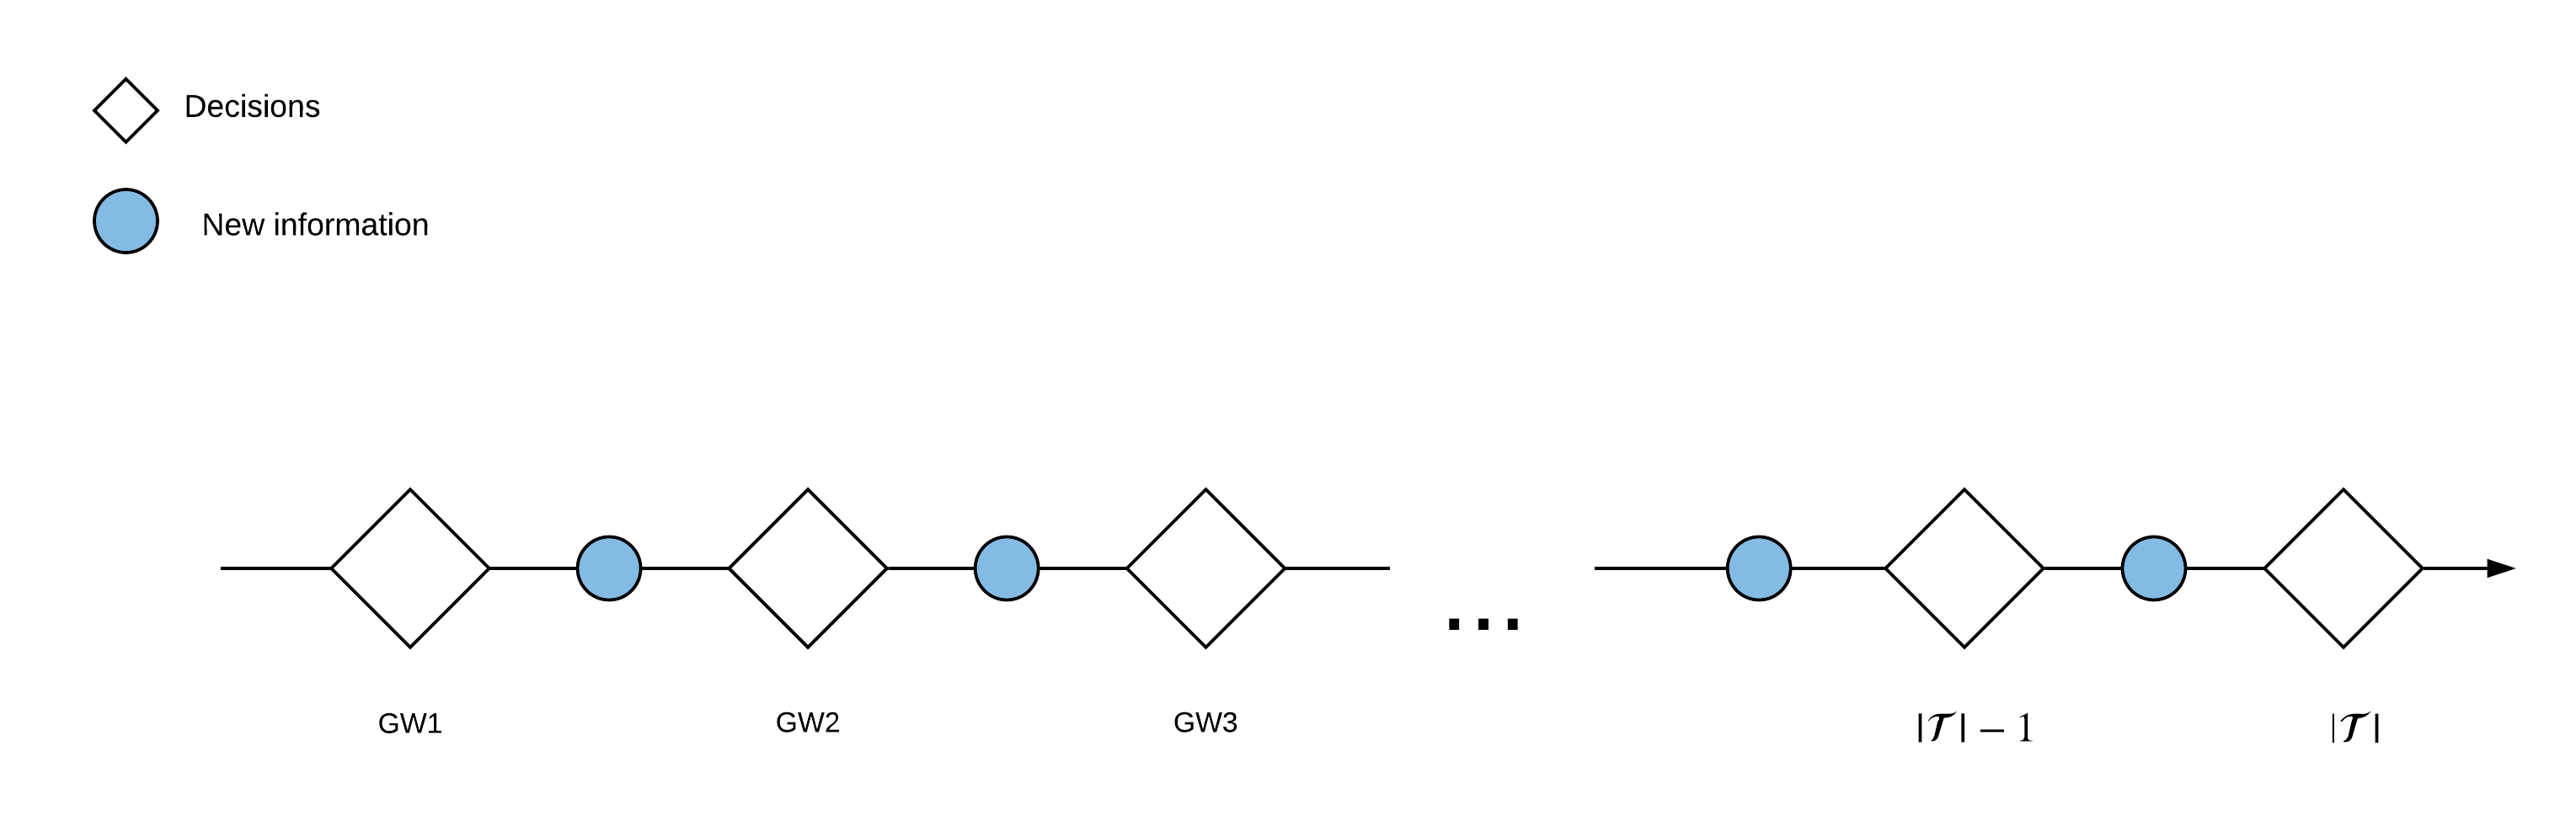
\includegraphics[scale = 0.47]{fig/chapter_5/Rolling_Horizon_Information_Flow.png}
    \caption{Information flow in the FPLDP.}
    \label{fig:information_flow}
\end{figure}

Rolling horizon is an appropriate solution method for FPLDP as managers are provided new information and face new decisions every gameweek. That is, each gameweek is a sub-problem. As shown in figure \ref{fig:information_flow}, decisions are made based on the information available. When a gameweek is played, updated information such as realized points, injuries and suspensions are made available. Hence, new decisions are made accordingly. Consequently, the problem is divided into $\mathcal{|T|}$ number of sub-problems along a time axis. That is, the decisions taken in a gameweek affect decisions in future gameweeks. However, decisions made early in the season have a limited impact on decisions made late in the season. It is fully possible to have a whole different selected squad in the last gameweeks compared to that of the first gameweeks. This is especially evident when the Wildcard is applied.

\newpar

In the rolling horizon heuristic, each sub-problem is solved over shorter sub-horizons. This corresponds well to the FPLDP, as FPL managers often consider several gameweeks when making decisions. Each sub-horizon is split in two time periods ($TP$). The two \textit{TP}s are $TP_k^{C}$, which is the central period that will be implemented in sub-problem $k$, and the forecasting period $TP_k^{F}$. Before solving sub-problem $k+1$, variables $x$, $v$ and $q$ are frozen prior to $k+1$ and used as input. The gameweek in which decisions are already implemented is regarded as the fixed period. The sub-horizon is shifted so that the first part of $TP_k^{F}$ becomes $TP_{k+1}^{C}$. If the central period and the forecasting period have equal length, the forecasting period becomes the new central period. To summarize, three periods are considered:

\begin{enumerate}[label=(\roman*)]
    \item \textbf{Fixed period (FP)}. A gameweek where decisions have been implemented and used as input for the next sub-problem. These decisions are the players that are selected in a gameweek, $x$, the remaining budget, $v$, and the number of free transfers available, $q$.
    \item \textbf{Central period (CP)}. A gameweek where new decisions are implemented. The decisions are which players to include in the selected squad, $x$, determining the starting line-up, $y$, the choice of captain, $f$,  vice-captain, $h$, whether to use a gamechip or not and which substitution priority, $g$, to assign.  
    \item \textbf{Forecasting period (PP)}. To avoid making too myopic decisions, a predefined number of gameweeks are selected and input data such as expected points are generated based on information available at that point in time. Decisions are made for these gameweeks, but not implemented.  The decisions are subject to change when new and updated information becomes available. 
\end{enumerate}

The FP, CP and PP in a sub-problem are illustrated graphically in Figure \ref{fig:rolling_horizon}. In the figure, the predicted part overlaps the central part in order to illustrate that the input data in the central part is also predicted. The sub-horizon is set to 4 gameweeks in the figure. 

\begin{figure}[H]
    \centering
    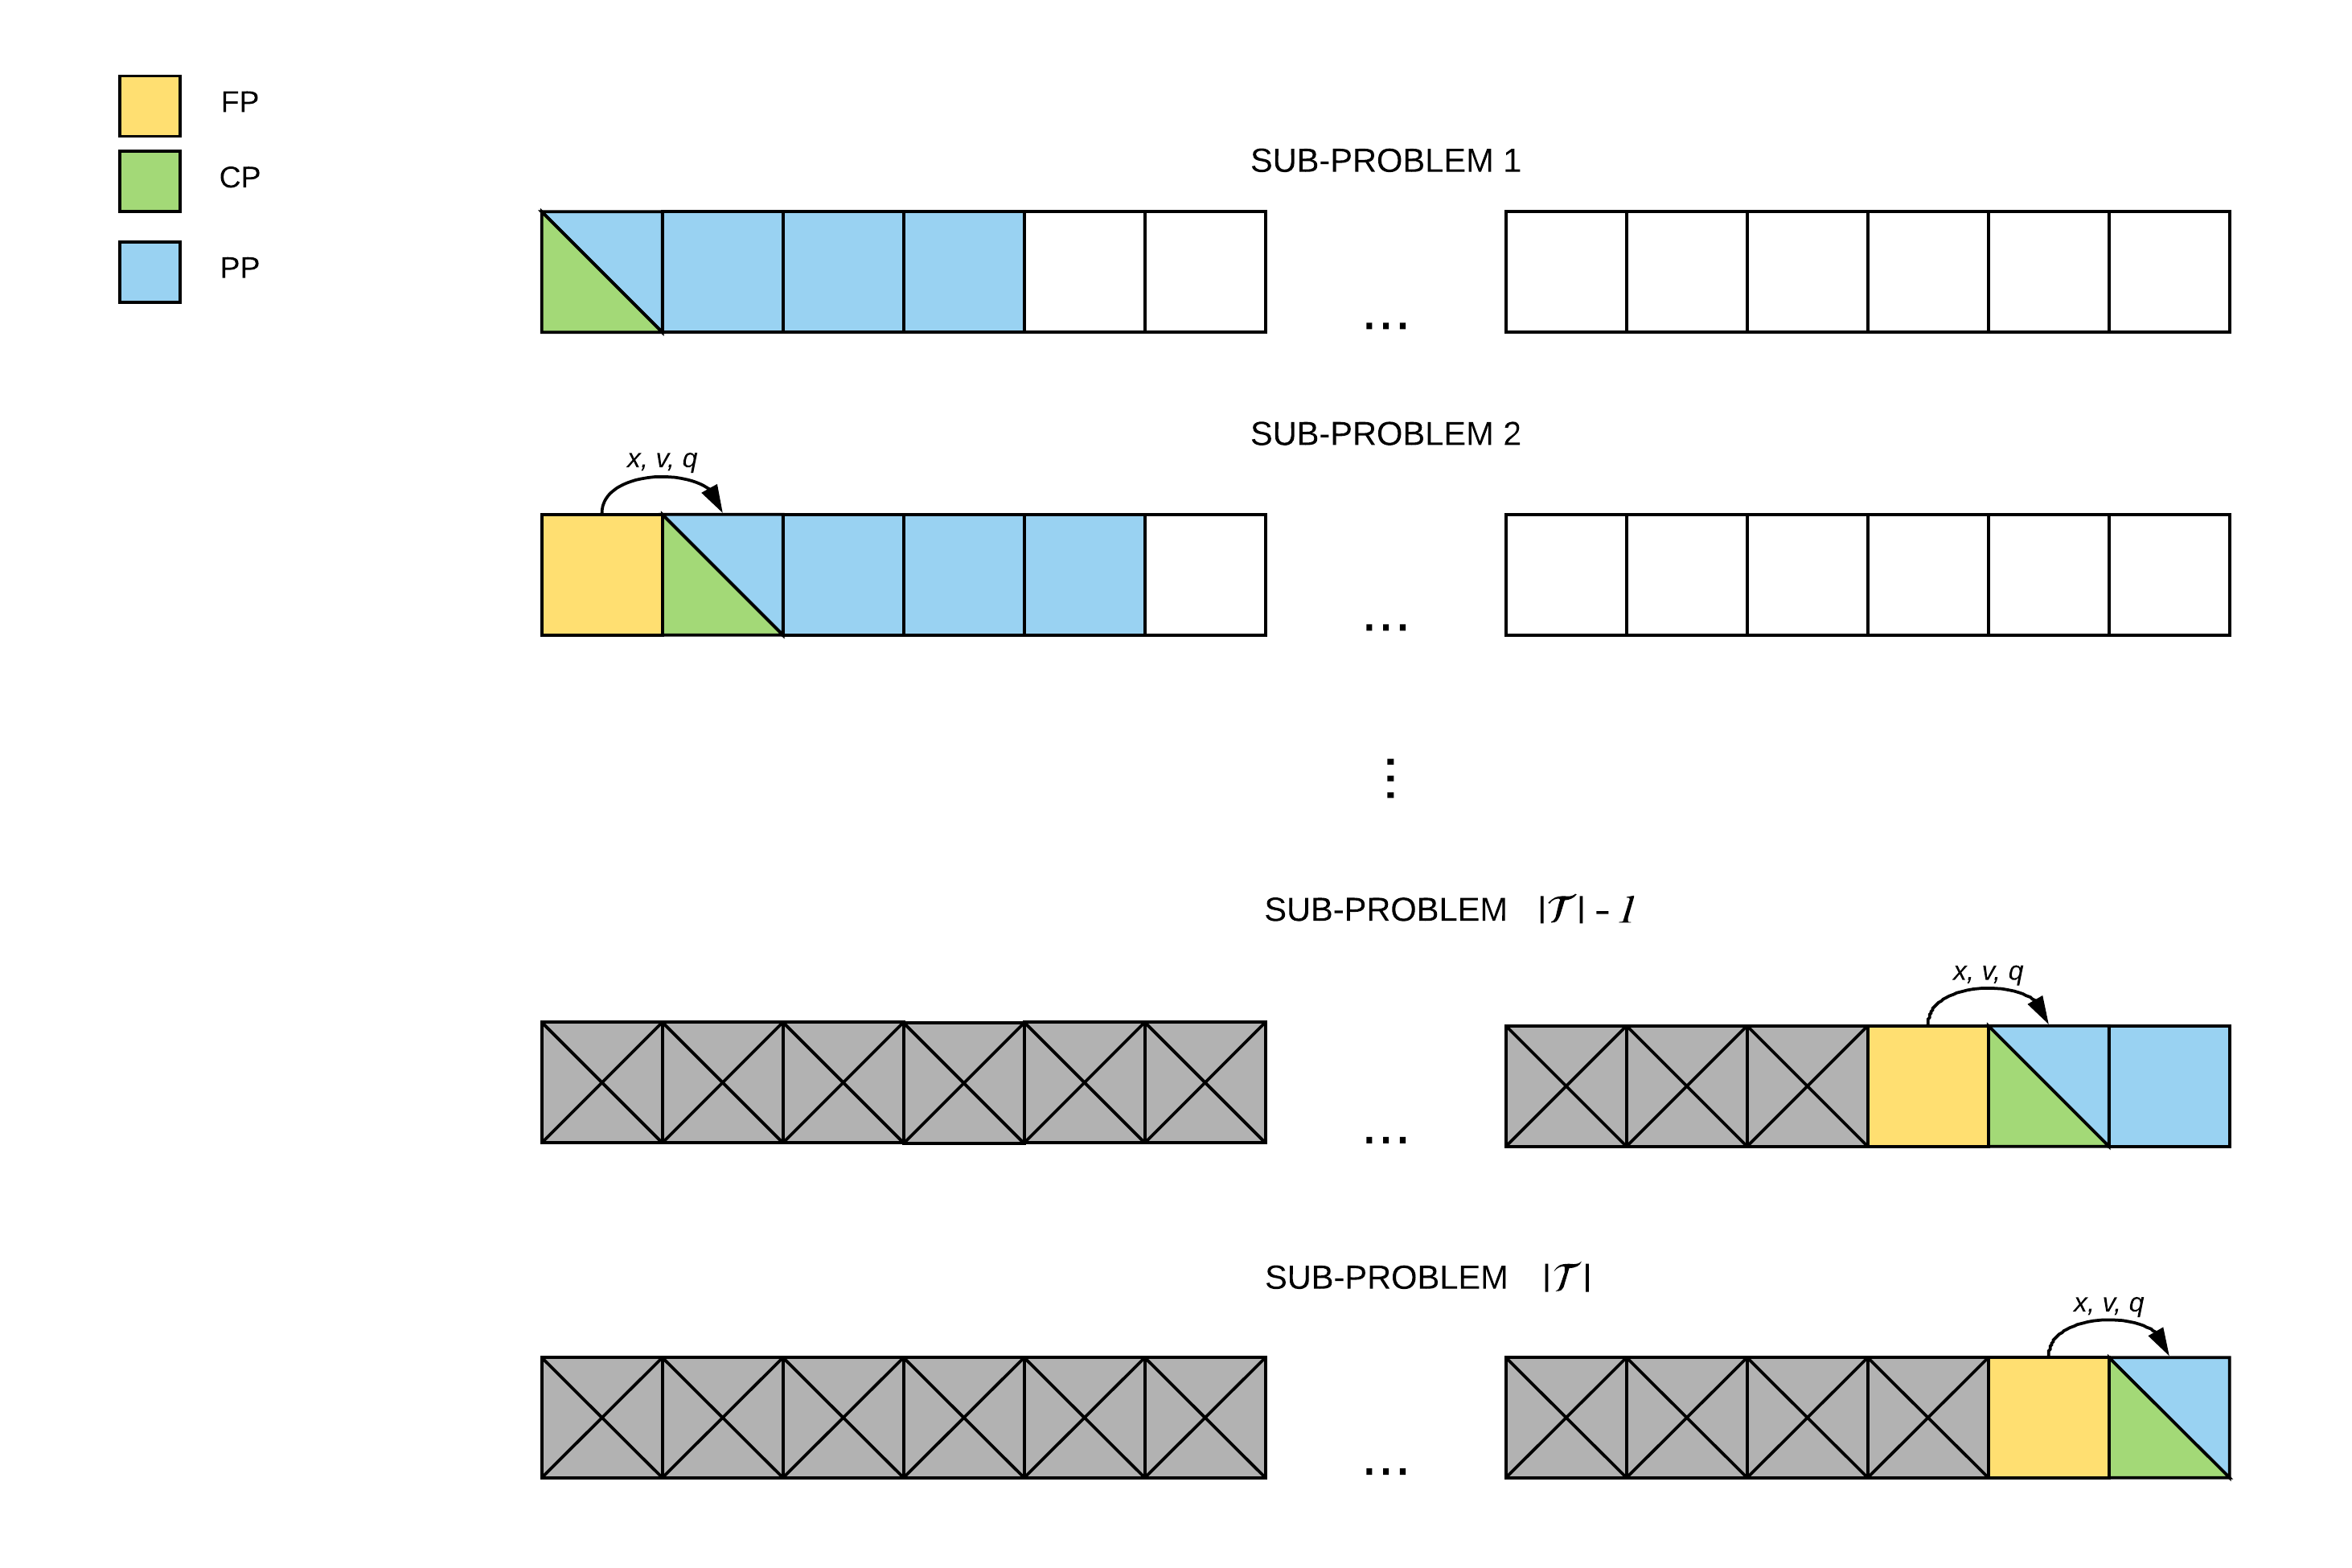
\includegraphics[scale = 0.47]{fig/chapter_5/rolling_horizon.png}
    \caption{Fixed-, central- and forecasting period in a sub-problem.}
    \label{fig:rolling_horizon}
\end{figure}

\newpar

An important decision is that of determining the length of the sub-horizon. Due to uncertainty in the forecasts, it is not necessarily ideal for the sub-horizon to be for the remaining length of the season. Thus, several alternatives concerning the length of the sub-horizon should be tested in order to see what gives the best result. In Chapter \ref{chapter_experimental_setup}, setting an appropriate length for the sub-horizon is further discussed. Note that in the framework, the aspect of value, sell price and sell-on fee with regards to a player's price is implemented. However, no attempt is made to forecast future prices. The prices are simply assumed to be what they are at the beginning of the horizon for the entire sub-horizon. For example, if the player Mahrez is bought for \pounds 9.0m in a sub-problem, his sell price is set to this for the sub-problem's entire sub-horizon. When solving for the next sub-problem, if his value increases to \pounds 9.2m, his sell price is updated to \pounds 9.1m and set to this for the entire sub-horizon. 

\section{Forecast of Player Points} \label{Player_Performance}

To generate input for the forecasting period in the rolling horizon heuristic, forecasts of player points are required. In this thesis, three forecasting methods are considered. The methods are: 

\begin{itemize}
    \item \textbf{Modified Average}. The solution approach suggested by \cite{Bonomo} is adapted and modified to FPL for prediction of a player's expected points.
    \item \textbf{Regression}. From a pool of explanatory variables related to the FPL, variables are selected and a linear regression model is fitted. 
    \item \textbf{Odds}. Bookmakers' odds can be transformed into a probability and consequently used to forecast future player points. Odds related to factors such as scorelines, goals and assists are utilized in order to estimate expected points. 
\end{itemize}


\subsection{Modified Average} \label{Sol_approach_Modified_Average}

As discussed in Section \ref{Forecasting_of_player_performance}, \cite{Bonomo} suggested a solution approach for the Argentinian Fantasy League and achieved promising results. Therefore, the first forecast method is based on their solution approach. However, the methodology is modified in order to make it applicable for the English Fantasy Premier League rather than the Argentinian Fantasy League. Moreover, some modifications are made as an effort to improve the method. Hence, the first forecasting method is called the Modified Average method.

\newpar

In Section \ref{Forecasting_of_player_performance} it is explained that  \cite{Bonomo} used the average points for the three last gameweeks to forecast player points in the upcoming gameweek. The forecast was further weighted by four factors: opponent strength factor, home-field advantage, whether a player is on a good performance streak and whether a player is assumed to be in the starting line-up. More specifically, \cite{Bonomo} estimated a player's expected points for the next gameweek according to Equation \ref{eq:bonomo}. In the following, it is explained how each factor of the equation was decided by \cite{Bonomo} and which modifications that are made.

\begin{equation}
\begin{split}
    \hat{\rho}  = & \textrm{\textit{Tracking average}} \times \textrm{\textit{ Opponent strength factor}} \times \textrm{\textit{Field factor}} \\
        & \times \textrm{\textit{Point streak factor}} \times \textrm{\textit{Starting line-up factor}}
\end{split}
\label{eq:bonomo}
\end{equation}


\newpage

\subsubsection{Tracking Average and Opponent Strength Factor}

\cite{Bonomo} calculated a \textit{tracking average} by averaging the points obtained in the 3 previous gameweeks. The first modification suggested is to consider averages over more than 3 previous gameweeks. The number of previous gameweeks taken into consideration when forecasting is hereby referred to as the \textit{track-length}. In addition, \cite{Bonomo} optimized for only 1 gameweek ahead when decisions are set in a current gameweek. Thus, \cite{Bonomo} used a sub-horizon of 1 gameweek and a track-length of 3 gameweeks when solving for the Argentinian Fantasy League.

\newpar

Considering different track-lengths is not the only modification made with respect to the tracking average. Another adjustment is to weigh previous points based on the strength of the opposition faced in the previous matches. \cite{Bonomo} did not account for the strength of the opposition faced when averaging previous points. However, they used league table position for measuring the relative strength between adversaries when predicting future points. That is, when they determined \textit{opponent strength factor}. Yet, league position suffers from numerous drawbacks which makes it unreliable for prediction. For example, the league table suffers from high variation in the early stage of the season and low variation in the late stage of the season. Further, competing teams may not share the equivalent number of matches during the season due to postponements. Additionally, the league table does not capture who has played against who during the season. Hence it is inherently biased until the final match of the season has been played \citep{Constantinou}. Therefore, instead of weighting the teams based on their league position, measuring team strength with basis in Elo rankings are suggested. 


\newpar

The Elo system, briefly introduced in Section \ref{Strength_of_football_teams}, is a rating system used for measuring the relative strength level of sports teams and individual athletes. Clubelo.com provides historical Elo ratings for most of the professional football teams in the world, including teams in the English Premier League. The Elo ratings provide a sophisticated measurement of the relative strength between the Premier League teams. Further, as the rating are updated once a match has been played, the Elo system considers the aspect of form. In addition, the ratings account for goal difference and inter-league adjustments. The Elo ratings also incorporate all fixtures, not only league matches. In Appendix \ref{A2_Elo_System}, it is shown how Elo ratings are transformed into a factor of team strength. 

\newpar


Once Elo ratings are obtained, they can be used in order to weight the previous points of each Fantasy Premier League player. In Table \ref{Elo.1617}, some Elo ratings for the first gameweeks of the English Premier League 2016/2017 season are listed. Note that the ratings are calculated ahead of each gameweek so that the ratings in the GW1 column are the Elo ratings of the teams before gameweek 1 has been played. 

\begin{table}[H]
\centering
\begin{tabular}{|l|l|l|l|l|l|}
\cline{2-6}
\multicolumn{1}{l|}{} & \multicolumn{1}{l|}{} & \multicolumn{4}{c|}{Elo rating}  \\ \cline{2-6} 
\hline
                      & Team                  & GW1    & GW2    & GW3  & GW4    \\
                      \hline
1                     & \Tstrut Chelsea               & 1793   & 1800   & 1798 & 1804   \\
2                     & Tottenham             & 1804   & 1804   & 1800 & 1798   \\
3                     & Man City              & 1848   & 1856   & 1858 & 1863   \\
4                     & Man Utd               & 1789   & 1797   & 1799 & 1804   \\
-                     &                       &        &        &      &        \\
-                     &                       &        &        &      &        \\
-                     &                       &        &        &      &        \\
17                    & Watford               & 1624   & 1631   & 1618 & 1612   \\
18                    & Hull                  & 1589   & 1603   & 1613 & 1608   \\
19                    & Middlesbrough         & 1595   & 1597   & 1601 & 1604   \\
20                    & Sunderland  \Bstrut          & 1655   & 1654   & 1636 & 1641   \\
\hline
\end{tabular}
\caption{Elo ratings for Premier League 2016/2017.}
\label{Elo.1617}
\end{table}


Ratings from Table \ref{Elo.1617} can be used in order to weight the previous points of a player. For instance, receiving 9 points against Chelsea is more impressive than receiving 9 points against Sunderland based in their respective Elo ratings. Hence, a suggestion is to weight the points accordingly. Equation \ref{eq:adj_avg} shows how a player's tracking average is computed when the track-length is $m$ and realized points in gameweek $i$ is denoted $\rho_i$. 

\begin{equation}
\textrm{\textit{Tracking average}} = \frac{1}{m}\sum_{i=1}^m \rho_i \cdot \frac{(\mathrm{Opponent \ Elo \ rating})_i}{(\mathrm{Team \ Elo \ rating})_i}
\label{eq:adj_avg}
\end{equation}

Furthermore, Elo ratings, rather than values based on the league table, are used to determine opponent strength factor, as seen in Equation \ref{eq:opp_str}. Thus, both previous points and future expected points account for faced and upcoming opposition. Notice that in Equation \ref{eq:adj_avg}, Elo ratings for both opponent and team is denoted with $i$. This is done because the Elo ratings are updated each gameweek.



\begin{equation}
\textrm{\textit{Opponent strength factor}} = \frac{\textrm{Team Elo rating}}{\textrm{Opponent Elo rating}}
\label{eq:opp_str}
\end{equation}


\subsubsection{Field Factor}
As pointed out in Section \ref{HomeFieldAdvantage}, numerous studies have concluded that a home-field advantage exists in football. That is, football teams have a tendency of performing better when playing at their home-field than when playing at an opponent's ground. In order to distinguish between home-field advantage and away-field (dis)advantage, the variable that takes such an advantage into account is called the \textit{field factor}. \cite{Bonomo} set the home-field factor to 1.05 and away-field factor to 0.95 without further elaboration. 

\newpar

Studies of home-field advantages in a football, e.g., \cite{Pollard}, usually concentrate on the outcome of the game, i.e., win, draw or loss. In Fantasy Premier League, however, the outcome of a match has no direct impact on the point system. Further, an important aspect influencing points in FPL is goals scored. Thus, the field factor is calculated with basis in goals. Further, the field factor is calculated for all teams in the Premier League combined, not for each team specifically. The idea is that the field factor alongside the relative team strengths calculated by the Elo ratings will complement each other. The home-field factor for a particular season is calculated as:

\begin{equation*}
    \textrm{Home-field factor} = \frac{\textrm{Total number of goals scored home}}{\textrm{Total number of goals scored}} 
\end{equation*}

Similarly, the away-field factor is calculated as:

\begin{equation*}
    \textrm{Away-field factor} = \frac{\textrm{Total number of goals scored away}}{\textrm{Total number of goals scored}}
\end{equation*}

As seen later in Section \ref{sec:comp_s_MA}, several previous seasons are considered in order to find an appropriate empirical value for the field factor.


\subsubsection{Point Streak Factor}

\cite{Bonomo} adjusted their forecasts with a value between 0.95 and 1.05 to account for a player's point streak. They did not further describe how the \textit{point streak factor} was determined. In this thesis, a player's point streak factor is determined in the following way: if a player receives more than \textit{X} points for 2 gameweeks in a row, his point streak factor will be set to 1.01. Further, if the streak continues, the factor will increase by 0.01 for each match that his points exceed \textit{X} number of points. When a player has received more than \textit{X} points 6 gameweeks in a row his point streak factor is set to the maximum of 1.05. Hence, the value does not increase if his streak exceeds 6 matches. The same rule applies to a player scoring less than \textit{Y} points 2 gameweeks in a row. In this case, his point streak factor will be set to 0.99. When obtaining less than \textit{Y} points 6 matches in a row the point streak factor is set to a minimum of 0.95. Once a streak is broken, the player's point streak factor is set to 1. In Section \ref{sec:comp_s_MA}, a method for determining \textit{X} and \textit{Y} is proposed.

\subsubsection{Starting Line-up Factor}

\cite{Bonomo} decided the \textit{starting line-up factor} by considering coaches' announcements, press reports and information posted on the website of the Argentinian Fantasy League. Such considerations are of qualitative nature. As the solution framework is intended to be data-driven, an explicit attempt at implementing this factor for the FPL is not undertaken. Instead, as seen later in Section \ref{exp_setup_data}, all forecasts are adjusted by data concerning injuries and suspensions.

\subsubsection{Summarizing Numerical Example}

In order to summarize the Modified Average method, a numerical example for a track length of 2 for Manchester United's Paul Pogba is provided. In Table \ref{tab:example_elo_ratings} and \ref{tab:example_realized_points}, fictive values for realized points and Elo ratings are given. 

\begin{table}[H]
\parbox{.45\linewidth}{
\centering
\begin{tabular}{|c|l|c|c|c|c|}
\hline
\multicolumn{1}{|c|}{} & \multicolumn{3}{c|}{Realized points} \\ \hline
Opponent       & GW1        & GW2       & GW3       \\
\hline                 
Chelsea  \Tstrut            & 6         &           &           \\
Sunderland             &           & 9         &           \\
Watford  \Bstrut         &           &           &  ?        \\
\hline
\end{tabular}
\caption{Realized points for Paul Pogba.}
\label{tab:example_realized_points}
}
\hfill
\parbox{.45\linewidth}{
\centering
\begin{tabular}{|l|c|c|c|}
\hline
Team        & GW1   & GW2   & GW3  \\ 
\hline
Man Utd  \Tstrut    & 1789  & 1797  & 1799  \\
Chelsea     & 1793  &       &       \\
Sunderland  &       & 1654  &       \\
Watford  \Bstrut    &       &       & 1618 \\ \hline
\end{tabular}
\caption{Elo ratings for three gameweeks.}
\label{tab:example_elo_ratings}
}

\end{table}

Thus, Paul Pogba's tracking average can be calculated as:

\begin{equation*}
    \textrm{Tracking Average} = \frac{1}{2} \cdot (6 \cdot \frac{1793}{1789} + 9 \cdot \frac{1654}{1797}) \approx 7.15
\end{equation*}


and the opponent strength factor can be found as:

\begin{equation*}
    \frac{1618}{1799} \approx 0.90
\end{equation*}

\begin{table}[H]
\centering
\begin{tabular}{|l|l|}
\hline
Factor   &  Value \\ 
            \hline
Tracking average \Tstrut &  7.15\\
Opponent strength factor & 0.90\\
Field factor  &  1.5 \\
Points streak factor  & 1 \\
Starting line-up factor \Bstrut & 1\\
\hline
\end{tabular}
\caption{Numerical values for Equation \ref{eq:bonomo}.}
\label{tab:example_modified_average}
\end{table}

Finally, all factors required to calculate the expected points for Paul Pogba in the upcoming gameweek are summarized in Table \ref{tab:example_modified_average}. Thus, in compliance with Equation \ref{eq:bonomo}, Pogba's expected points for the upcoming gameweek are according to the Modified Average method:

\begin{equation*} \label{eq:pogba_ma}
    7.15 \cdot 0.90 \cdot 1.5 \cdot 1 \cdot 1 \approx 9.7
\end{equation*}




\subsection{Regression}
\label{Sol_approach_regression}

As seen in the literature review, regression is commonly in research related to sports (\cite{vabo}; \cite{Yang}). Therefore, as a second way of forecasting Fantasy Premier League points, a regression-based method is proposed. In order to create a regression model, the following steps are undertaken:

\begin{enumerate} [label=(\roman*)]
    \item separate players based on position,
    \item perform a variable selection,
    \item fit a linear regression model.
\end{enumerate}

\subsubsection{Variables}
In order to use regression to estimate expected points, numerous numerical and categorical explanatory variables are considered. In the following, all variables considered are presented: 

\newpar

\textbf{Dependent Variable}
\begin{itemize}
    \item \textbf{Realized points} - The dependent variable. The realized points are the actual points gained by players.
\end{itemize}

\textbf{Explanatory Variables}

\textit{Categorical Variables}
\newpar
\begin{itemize}
    \item \textbf{Team} - Which teams the players play for. This variable can change during the international transfer window in August and January.  
    
    \item \textbf{Position} - Describes whether a player is a goalkeeper, defender, midfielder or forward. The variable is constant throughout the season.
    \item \textbf{Home/Away} - Displays whether a match is played at home or away.
\end{itemize}
\newpar

\textit{Numerical Variables}
\newpar
\begin{itemize}
    \item \textbf{Previous points} - Points obtained in the previous gameweeks.
    \item \textbf{Price} - The purchase price (value) of a player.
    \item \textbf{Transfers in} - The amount of FPL managers that bought the player ahead of a given gameweek.
    \item \textbf{Transfers out} - The amount of FPL managers that sold the player ahead of a given gameweek.
    \item \textbf{Minutes Played} - Minutes played in the previous gameweek.
    \item \textbf{Yellow Cards} - Total amount of yellow cards received in the previous gameweeks.
    \item \textbf{Red Cards} - Total amount of red cards received in the previous gameweeks.
    \item \textbf{Goals} - Total amount of goals scored in the previous gameweeks.
    \item \textbf{Assists} - Total amount of assists in the previous gameweeks.
    \item \textbf{Penalties Missed} - Total amount of penalties missed in the previous gameweeks.
    \item \textbf{Penalties Saved} - Total number of penalties saved by a goalkeeper in the previous gameweeks.
    \item \textbf{Saves} - Total amount of saves made by a goalkeeper in the previous gameweeks.
    \item \textbf{Clean sheets} - Total number of matches a player was awarded a clean sheet in the previous gameweeks. As explained in Chapter \ref{chapter_problem_description}, clean sheets are only awarded goalkeepers, defenders and midfielders who play a minimum of 60 minutes during the match.
    
\end{itemize}

\subsubsection{Categorization by Position}

%Seperate analysis by positions because of different eccects of covariates (betas)

As described in Chapter \ref{chapter_problem_description}, points are awarded based on different criteria to players in different \textit{positions}. For instance, goalkeepers, defenders and midfielders are rewarded points for keeping a clean sheet, but forwards are not. Based on this knowledge, it is decided to categorize the players based on their respective positions before continuing the regression procedure. If all available variables were regressed, such a distinction would perhaps not be necessary, as the coefficient related to the categorical variable position could compensate the differences. However, the aim is to limit the number of explanatory variables for each position by use of variable selection. Therefore, the categorization is done. 

\newpar

In order to provide further justification for the categorization based on position, a box-plot and scatter-plots are assessed in Section \ref{exp_setup_reg}. For example, in the box-plot, it is investigated whether the empirical distribution of points obtained differs between positions. Moreover, the scatter plots are visually inspected to see the relation between, for example, total points, goals and position.

\subsubsection{Times Series Effect of Points}

The presence of a scoring streak, or a "hot hand", has long been a topic of research (\cite{hot_hand}; \cite{hot_hand_2}). If it is present in FPL, points gained in the most previous matches could be an interesting explanatory variable. If not, aggregated variables such as the total number of goals scored can be just as predictive. In order to assess if elements of a time series are correlated with each other, \textit{autocorrelation} is a reasonable metric to asses. Just as correlation measures the extent of a linear relationship between two variables, autocorrelation measures the linear relationship between lagged values of a time series \citep{Hyndman}. For example, $r_1$ measures the relationship between $y_t$ and $y_{t-1}$. In general, there exist many autocorrelation coefficients, and the value of $r_k$ can be written as in Equation \ref{eq:rk}. 


\begin{equation}\label{eq:rk}
    r_k = \frac{\sum_{t=k+1}^T(y_t-\bar{y})(y_{t-k}-\bar{y})}{\sum_{t=1}^T(y_t-\bar{y})^2}
\end{equation}

To test for autocorrelation, the Ljung-Box test and the Durbin-Watson test are conducted. The Ljung-Box test is a statistical test that often is conducted in order to test for autocorrelation in a time series for different lags \citep{Hyndman}. The Durbin-Watson test is another test frequently conducted to test for the presence of autocorrelation for the first lag \citep{Carol_1}. A detailed description of the tests can be found in \cite{Hyndman} and \cite{Carol_1}, respectively.

\subsubsection{Variable Selection}

In order to select variables, \textit{k-fold cross validation} is performed in combination with a \textit{lasso regression}. Before these topics are treated, a brief discussion of training- and test sets and forecast error measurement is presented.


\subsubsection{Training- and Test Sets}
In general, in order to determine the accuracy of a forecast, out-of-sample forecasts should be evaluated \citep{Hyndman}. To accomplish this, available data should be separated into two portions: training- and test data. A model is first fitted using the training data only. Then, the model's forecast accuracy is determined by comparing forecasts from the model with actual realizations contained in the test data. Furthermore, in general, if a model is fit on all available data, rather than separated into a training- and test set, the model would be subject to over-fitting \citep{Hyndman}. That is, the model performs well on the sample data but does not necessarily forecast well out of sample.

\subsubsection{Forecast Error Measurement}
A forecast error is the difference between an observed value and its forecast \citep{Hyndman}, as defined as in Equation \ref{eq:f_err}. Here, \{$ y_{1},...,y_{T} $\} is the training set data, \{$ y_{T+1},,y_{T+2},...$\} is the test set data and $\hat{y}_{t+h|T}$ is the forecast at time \textit{T+h}, given \textit{T}. 

\begin{equation}\label{eq:f_err}
    e_{T+h} = y_{T+h} - \hat{y}_{T+h|T}
\end{equation}

Commonly used error measures include the Mean Squared Error (MSE, Equation \ref{eq:MSE}) and Root Mean Squared Error (RMSE, Equation \ref{eq:RMSE}) \citep{Hyndman}.

\begin{equation}\label{eq:MSE}
    MSE = mean(e_t^2)
\end{equation}

\begin{equation}\label{eq:RMSE}
    RMSE = \sqrt{MSE}
\end{equation}


\subsubsection{\textit{k}-fold Cross Validation}
\textit{k}-fold cross validation involves randomly dividing a set of observations into \textit{k} groups, or \textit{folds}, of equal size \citep{ISLR}. The first fold is treated as the test set, and the remaining $k-1$ folds are used to train a model. The procedure is repeated \textit{k} times, and for each repetition, a new fold makes up the test set. The process results in \textit{k} estimates of the test-error, $MSE_1$, $MSE_2$ ..., $MSE_k$. Finally, a \textit{k}-fold average MSE, denoted $CV_{(k)}$ is computed by averaging the values, as shown in Equation \ref{eq:cv} \citep{ISLR}.

\begin{equation}\label{eq:cv}
    CV_{(k)} = \frac{1}{k}\sum_{i=1}^{k} MSE_i
\end{equation}

\subsubsection{Lasso Regression}

As seen previously, a number of explanatory variables are available. If all were to be used to build a regression model, the model could be subject to over-fitting \citep{ISLR}. Therefore, in order to limit the number of explanatory variables, a \textit{variable selection} is undertaken. That is, a subset of variables believed to be related to the dependent variable \textit{realized points}, is selected. To perform the variable selection, lasso regression is used. In this thesis, only a brief introduction of the concept of lasso regression is given. For a more comprehensive review, the reader is referred to "An Introduction to Statistical Learning" by \cite{ISLR}.

\newpar

According to \cite{ISLR}, lasso regression is a \textit{shrinkage method} used in order to perform variable selection. By shrinkage method, the authors refer to methods were coefficients are sunken towards zero relative to least squares estimates. This shrinkage has the effect of reducing variance. Depending on what type of shrinkage is performed, some of the coefficients may be estimated to be exactly zero. Lasso regression is such a shrinkage method and can thus perform variable selection. The aim of lasso regression is to find the lasso coefficients $\hat{\beta}_{\lambda}^{L}$ by minimizing the expression found in Equation \ref{eq:lasso}:

\begin{equation}
    \sum_{i=1}^n\Big (y_i-\beta_0-\sum_{j=1}^p\beta_jx_{ij}\Big)^2 + \lambda \sum_{j=1}^p|\beta_j| = RSS + \lambda \sum_{j=1}^p|\beta_j|
    \label{eq:lasso}
\end{equation}

Here, RSS is the Residual Sum of Squares, which is minimized in multiple linear regression. However, in contrast to linear regression, Lasso regression does not only minimize RSS. It also penalizes the sum of the $\beta$-coefficients by absolute value. Or, more precisely, it uses an $l_1$ penalty. This has the desired effect of forcing some of the coefficient estimates to be exactly equal to zero when the tuning parameter $\lambda$ is sufficiently large \citep{ISLR}. Hence, lasso regression performs a variable selection.

\newpar 

In order to decide the value of $\lambda$, and subsequently what variables to include in the model, \textit{k}-fold cross validation is used. In Section \ref{exp_setup_reg}, the average \textit{k}-fold cross validation MSE, $CV_{(k)}$, associated with the coefficients $\hat{\beta}_{\lambda}^{L}$, is plotted against corresponding values of $\lambda$. As suggested by \cite{ISLR}, two considerations are made when selecting a value of $\lambda$. First, the model with the smallest error is considered. However, if such a model includes a large number of explanatory variables, it can be subject to over-fitting. Therefore, the model with an MSE one standard deviation higher than that of the minimum is also considered. Afterwards, a variable selection is performed. That is, the variables associated with a non-zero $\hat{\beta}_{\lambda}^{L}$ are chosen. 

\subsubsection{Model Selection}

It is important to note that lasso regression is only conducted in order to perform variable selection. The  $\hat{\beta}_{\lambda}^{L}$-values from the regression are \textit{not} carried forward. Instead, points are forecast by use of linear regression on the variables selected by the lasso regression. Linear regression has an advantage over a lasso regression as it has more easily interpreted coefficients and well-defined variance \citep{ISLR}. This makes the calculation of \textit{p}-values possible. Moreover, the use of linear regression makes the results more accessible to readers from different disciplines as it is a widely known procedure. Furthermore, a linear regression model has an advantage compared to for instance logistic regressions as points can be negative, which is a possibility in FPL.

\newpar 

The variable \textit{previous points} is the only variable explicitly related to points earned. Other variables such as total points in the season so far and points from the Bonus Point System are not included. These variables would be highly correlated with variables such as goals. Thus, one rationale for excluding them is not to over-complicate the correlation between explanatory variables in the regression model. Furthermore, since the bonus points are to a substantial degree decided by the same factors as "regular" points (e.g., goals, assists, clean sheets etc.), their effects are assumed included in the coefficients for these explanatory variables. 


\subsection{Odds}

As seen in the literature review in Section \ref{Strength_of_football_teams}, \cite{Hvattum} found that Elo ratings appeared to be considerably less accurate than market odds when used for forecasts. Furthermore, in their project report, \cite{Gupta} created a scoreline prediction for the fixtures of the Premier League and used it in order to forecast future performance of the players in FPL. However, they found their scoreline predictions far less accurate than those of bookmakers' odds. Therefore, it interesting to adopt an approach based on bookmakers' odds, as the method is complementary to the Elo based Modified Average method.


\newpar

In order to obtain predictions of player points, odds must be transferred into expected points. Odds can be separated into \textit{team odds} and \textit{individual player odds}. Team odds include all odds related to a team's performance such as result odds. Individual player odds include odds related to an individual player's performance such as goals scored, assists provided and bookings. 

\newpar

The team odds used is related to scorelines and serve two purposes. First, it is used to calculate the probability of a team keeping a clean sheet. By summing all the result odds and dividing each individual result odds by that sum, the probability of each exact result can be obtained. In Table \ref{tab:odds_probabilities}, an example is given for the odds and the corresponding probabilities. By summing all the probabilities for the scorelines where Leicester has a clean sheet, it can be found that the probability of Leicester keeping a clean sheet is 0.316. Thus, in order to calculate expected points from clean sheets, the probability is multiplied with points received for a clean sheet, i.e., 4 points for goalkeepers and defenders and 1 point for midfielders. Secondly, team odds is used to obtain a team's expected goals. This is done by multiplying goals scored in each scoreline with the probability of that scoreline occurring. In the example from Table \ref{tab:odds_probabilities} Leicester's expected goals is found to be 1.310.


\begin{table}[H]
\begin{subtable}{1\textwidth}
\centering
\begin{tabular}{|lc|lc|lc|}
\multicolumn{6}{c}{Odds}                   \\
\hline
1-0 & 7.00 \Tstrut   & 0-0 & 7.50   & 0-1 & 8.00   \\
2-0 & 11.00  & 1-1 & 6.00   & 0-2 & 13.00  \\
2-1 & 9.50   & 2-2 & 15.00  & 1-2 & 10.50  \\
3-0 & 23.00  & 3-3 & 67.00  & 0-3 & 29.00  \\
3-1 & 21.00  & 4-4 & 301.00 & 1-3 & 23.00  \\
3-2 & 31.00  &     &        & 2-3 & 35.00  \\
4-0 & 61.00  &     &        & 0-4 & 81.00  \\
4-1 & 56.00  &     &        & 1-4 & 67.00  \\
4-2 & 81.00  &     &        & 2-4 & 91.00  \\
4-3 & 181.00 &     &        & 3-4 & 201.00 \\
5-0 & 201.00 &     &        & 0-5 & 276.00 \\
5-1 & 181.00 &     &        & 1-5 & 226.00 \\
5-2 & 276.00 \Bstrut  &     &        &     &        \\
\hline
\end{tabular}
\end{subtable}
\bigskip
\begin{subtable}{1\textwidth}
\centering
\begin{tabular}{|ll|ll|ll|}
\multicolumn{6}{c}{Probabilities}                         \\
\hline
1-0 \Tstrut  & 0.1043 & 0-0 & 0.0974 & 0-1 & 0.0913  \\
2-0 & 0.0664 & 1-1 & 0.1218 & 0-2 & 0.0562 \\
2-1 & 0.0769 & 2-2 & 0.0487 & 1-2 & 0.0696 \\
3-0 & 0.0318  & 3-3 & 0.0109 & 0-3 & 0.0251 \\
3-1 & 0.0348 & 4-4 & 0.0024 & 1-3 & 0.0318  \\
3-2 & 0.0236 &     &          & 2-3 & 0.0209 \\
4-0 & 0.0120 &     &          & 0-4 & 0.0090 \\
4-1 & 0.0130 &     &          & 1-4 & 0.0109 \\
4-2 & 0.0090 &     &          & 2-4 & 0.0080  \\
4-3 & 0.0040 &     &          & 3-4 & 0.0036 \\
5-0 & 0.0036 &     &          & 0-5 & 0.0026 \\
5-1 & 0.0040 &     &          & 1-5 & 0.0032 \\
5-2 \Bstrut  & 0.0026 &     &          &     &         \\
\hline
\end{tabular}
\end{subtable}
\caption{Result odds for Leicester-Burnley 14.04.18 and the corresponding probabilities.}
\label{tab:odds_probabilities}
\end{table}



In an analogous manner as with team odds, individual odds can be transformed into probabilities. However, now the probabilities are calculated as the inverse of the odds. Thus, if Leicester's Riyad Mahrez is assigned an odds of 4 for scoring one or more goals, his probability of scoring is $\frac{1}{4}=25\%$. Note, however, that by using this method it is assumed that the odds are set in a "fair" way, i.e., the odds market is a perfect market. In reality, bookmakers are profit-seekers. Thus, if bookmakers are to profit, the odds they set must transfer into probabilities lower than the real ones, and the validity of assumption can be weakened. After odds are transferred into probabilities, the probabilities are converted to expected points. For points related to scoring a goal, for example, this is achieved by multiplying expected goals and points obtained for a goal. Points for assists are allocated in a similar manner. Note, that not all goals are assisted. However, it is assumed that bookmakers consider this when setting the odds.

\begin{table}[H]
\centering
\begin{tabular}{|lcc|}
\hline
            & Odds & Probability \\ \hline
Goal    \Tstrut    & 4    & 0.25        \\
Assist      & 2.5  & 0.40        \\
Yellow Card \Bstrut & 8    & 0.125       \\ \hline
\end{tabular}
\caption{Fictive individual odds for Riyad Mahrez.}
\label{tab:ind_odds_riyad_mahrez}
\end{table}


Finally, the expected points of a player can be computed. In Table \ref{tab:ind_odds_riyad_mahrez}, a fictive set of individual odds and probabilities are given for the Leicester midfield player, Riyad Mahrez. The reader is reminded that a midfielder earns 5 points for a goal, 3 points for an assist, 1 point for a clean sheet and -1 point for a yellow card. In equation \ref{eq:riyad_mahrez_odds}, it is shown that he is expected to obtain 3.40 points for the Leicester-Burnley match.


\begin{equation} \label{eq:riyad_mahrez_odds}
    5 \cdot 1.310 \cdot 0.25 + 3 \cdot 1.310 \cdot 0.4 + 1 \cdot 0.316 - 1 \cdot 0.125 \approx 3.40
\end{equation}

Note that the probability of starting is not explicitly handled. Nor is points awarded for playing over 60 minutes. However, one can argue that the probability of starting is incorporated in individual odds, i.e., as the probability of scoring a goal or providing an assist.

\section{Gamechips} \label{Ch.5_Game_chips}

Gamechip strategies are actions developed to decide when it is optimal to use the gamechips. There exists limited literature on this topic. Consequently, there is a leeway for new ideas. Many interesting approaches could be adopted to decide the optimal use of gamechips. The approach adopted in this thesis is mainly qualitative and aim to take advantage of future gameweeks which are \textit{blank} or \textit{double}. The reader is reminded gameweek is blank when at least one team does not play, and a double if a team is featured more than once. 

\newpar

FPL managers must make decisions on when to use their gamechips, i.e., they have to decide whether it is best to play them in a given gameweek or if it is optimal to wait. As the model is solved using a rolling horizon heuristic, a strategy for when to use the gamechips is required. Since the model is solved over a sub-horizon, there is nothing that prevents the model from not using the gamechips in the current sub-problem, unless the strategy addresses this issue. Many different approaches can be undertaken to develop such a strategy. One strategy is to base the decisions on intuition and well-known strategies among FPL managers.\footnote{See websites \url{https://www.premierleague.com/news/624013} and \url{https://www.premierleague.com/news/404004}} As limited research is conducted on the use of gamechips, these strategies are considered an appropriate place to start. Other interesting approaches include to consider a type of punishment in terms of penalized points for the use of gamechips or to implement the gamechips analogous to the exercise of a financial option. Thus, strategies that are more quantitatively influenced are exciting topics for future research.

\subsection{First Wildcard}

The first Wildcard, which has to be played within the first half of the season, is played at the end of the first quarter of the season. There is high uncertainty at the start of the season related to starting line-ups and the form of players. In addition, the summer transfer window ends in gameweek 4, providing a possibility of players being sold, lend or bought. Thus, using the Wildcard after a few gameweeks allows managers to wait and consider such developments. However, if managers wait too long, they can miss the opportunity of adding players that over-perform compared to their initial expectations. Hence, playing the Wildcard in last part of the first quarter of the season takes both considerations into account. This is implemented by giving the mathematical model the opportunity to play a Wildcard in a specific gameweek which is chosen beforehand.

\subsection{Triple Captain}
It is assumed sensible to play the Triple Captain in a double gameweek as players are expected to gain more points when they are featured twice. Thus, the model is given the opportunity to play the Triple Captain in the first double gameweek of the season. 

\subsection{Second Wildcard and Bench Boost}
The second Wildcard should be played with caution, as it is wise also to consider the Bench Boost when using it. As the Bench Boost allows each player in the selected squad to collect points, and not only the starting line-up, the Bench Boost should be played in a double gameweek. Therefore, the model is set to play the second Wildcard in the gameweek ahead of a double gameweek.


\subsection{Free Hit}
The Free Hit allows a manager to perform an unlimited amount of free transfers for one gameweek. In the gameweek after, the selected squad is changed back. There are in general two cases where playing the Free Hit is reasonable. First, the Free Hit could be played in a blank gameweek to ensure that all the players in the starting line-up are featured for that particular gameweek. Second, the Free Hit could be played in a double gameweek to ensure that the majority of the starting line-up consists of players that are featured twice. As two other gamechips already are related to double gameweeks, the first method is implemented.

\subsection{Gamechip Implementation in the Mathematical model}

The gamechips are implemented in the mathematical model by initially setting the right-hand side of constraints \ref{eq:wildcard_first_half_of_the_season} - \ref{eq:free_hit} equal to 0. The right-hand side of the constraints is only set to 1 in the respective constraints when a gameweek where a gamechip can be played is considered in the sub-horizon. Up to those gameweeks, the constraints are deactivated and have no effect on the objective function.

\newpar

The opportunity of using a gamechip is first introduced when reaching a sub-horizon which includes a gameweek where a gamechip can be used. When that particular gameweek is reached, the related constraints are split in two. For example, if the sub-horizon is set to 4, and the first Wildcard is allowed to be played in gameweek 12, it is first considered when the mathematical model is run for sub-problem 9. In the model, the right-hand side of constraints \ref{eq:wildcard_second_half_of_the_season} - \ref{eq:free_hit} are set to 0, while constraints \ref{eq:wildcard_first_half_of_the_season} is split in two: 

\begin{equation*}
    \begin{aligned}
      \sum_{t \in \{9,10,11 \}} w_{t} & \leq 0 \\
         w_{12} & \leq 1
    \end{aligned}
\end{equation*}

In the next sub-problem, the range is moved so the constraints is now modelled as: 

\begin{equation*}
    \begin{aligned}
      \sum_{t \in \{10,11,13\}} w_{t} & \leq 0 \\
         w_{12} & \leq 1
    \end{aligned}
\end{equation*}

The other gamechips are implemented in a similar way as the Wildcard. 



\section{Risk Handling} \label{Ch.5_Variance_tradeoff}

As both goalkeepers and defenders in the same team earn 4 points for keeping a clean sheet, it is not hard to imagine that the points they obtain are positively correlated. Similarly, it is not unreasonable to assume that the points a goalkeeper and forward of opposing teams earn are negatively correlated. In this section, a method for dealing with this assumed correlation in points obtained, as well as the fluctuations of individual player's points, is presented. As described in Section \ref{Other_Relevant_Research}, there is a large resemblance between the FPLDP and the well-known portfolio selection problem in financial optimization. This is taken advantage of as risk is handled in an analogous manner. Thus, one might say that the objective of adding risk handling is \textit{diversification}, a risk management technique with the purpose of yielding higher returns (expected points) without increasing risk.



\subsection{Player Variance}

Variance refers to the variability in each player's realized points. Some midfielders are for instance known to be consistently starting but seldom contribute in terms of assists or goals. It is reasonable to assume that such players have a low expected value of points, but also a low variability in points obtained. Other players might contribute a lot in terms of assists and goals when they are playing, but are perhaps often injured. Such players could have a high predicted value, but also a high variance in points obtained.

\subsection{Correlation}

The variance of each player only considers each player's individual contribution to the team's total variance. As discussed, it is natural to assume that there exists a correlation between the points obtained by players. However, even if the points obtained by a goalkeeper and a defender from the same team are expected to be positively correlated, it is perhaps not so obvious whether or not there exists correlation between defenders of opposing teams. In order to test for correlation, Pearson's Product-Moment Correlation test is performed. By applying the test, a few assumptions are made. The variables are assumed approximately normally distributed and display \textit{homoscedasticity} (constant variance). For a full description of Pearson's Product-Moment Correlation test and its underlying assumptions, the reader is referred to \cite{laerd}.

\subsection{Team Variance}

In financial optimization, it is common to examine the trade-off between expected return and variance \citep{Markowitz}. According to \cite{Zenios}, the variance of a portfolio containing \textit{n} assets with weight \textit{w} can be expressed as 

\begin{equation}
    \sigma^2(w) = \sum_{i = 1}^{n}\sum_{i' = 1}^{m}\sigma_{ii'}w_{i}w_{i'} = \sum_{i = 1}^{n}\sigma_{i}^2w_i^2 + \sum_{i = 1}^{n}\sum_{\substack{i' = 1;\\ i' \neq i}}^{n}\sigma_{ii'}w_iw_{i'}
    \label{eq:port_var}
\end{equation}

where, $w_i$ is the portfolio weight of asset $i$, $\sigma_{i}^2$ is the variance of asset \textit{i} and $\sigma_{ii'}$ is the covariance between assets $i$ and $i'$. 

\newpar

In the case of FPLDP, the mathematical model optimizes over the starting line-up variable, $y$. In Equation \ref{eq:port_var} returns are expressed in percentage, as is common in finance.  
For the FPLDP, however, it is the variance of the sum of total points obtained each gameweek, rather than the variance in percentage return, that is of interest. Hence, Equation \ref{eq:port_var} can be rewritten by utilizing the fact that each "portfolio weight" is either 1 or 0. If the expression for covariance is also substituted with correlation, the expression simplifies to


\begin{equation}
    \sigma^2(y) = \sum_{i = 1}^{n}\sigma_i^2y_i + \sum_{i = 1}^{n}\sum_{\substack{j = 1;\\ j \neq i}}^{n} \sigma_i^{2}\sigma_j^{2}y_{i}y_{j}\eta_{i,j}
    \label{eq:team_var}
\end{equation}

where $\sigma_{i}^2$ is the variance of expected points obtained by player \textit{i}, $\sigma_{j}^2$ is the variance of expected points obtained by player \textit{j} and $\eta_{i,j}$ is the correlation between expected points obtained by player $i$ and player $j$. In addition, $y_i$ and $y_j$ are binary variables indicating whether player $i$ and player $j$ are included in the starting line-up (portfolio) of players. Conventionally $\rho$ is used to denote correlation. However, in this thesis, $\eta$ denotes correlation as $\rho$ is already reserved for denoting points.

\newpar

In the mathematical model, an upper threshold is determined for the variance of the starting line-up at time $t$ as described below. Note that in Equation \ref{eq:team_var} two binary variables are multiplied. In order to linearize the expression, an auxiliary variable, $\delta_{pp't}$, is introduced and the following set of equations are inferred.

\begin{equation} \label{eq:variance}
    \sigma^2_{t} = \sum_{p = 1}^{P}\sigma_p^2 y_{pt} + \sum_{p = 1}^{P}\sum_{\substack{p' = 1; \\ p' \neq p}}^{P} \sigma_p^2\sigma_{p'}^2\eta_{p,p',t} \delta_{pp't} \qquad\qquad t \in \mathcal{T}
\end{equation}

\begin{equation} \label{eq:variance_threshold}
    \sigma^2_{t} \leq \sigma_{0}^2 \qquad\qquad t \in \mathcal{T}
\end{equation}

\begin{equation} \label{eq:variance_p_beta}
    \delta_{pp't} \leq y_{pt}  \qquad\qquad p \in \mathcal{P}, p' \in \mathcal{P}, p' \neq p, \enskip t \in \mathcal{T}
\end{equation}

\begin{equation} \label{eq:variance_p_dash_beta}
    \delta_{pp't} \leq y_{p't}  \qquad\qquad p \in \mathcal{P}, p' \in \mathcal{P}, p' \neq p, \enskip t \in \mathcal{T}
\end{equation}

\begin{equation} \label{eq:variance_p_p_dash_beta}
    \delta_{pp't} \geq y_{pt} + y_{p't} - 1  \qquad\qquad p \in \mathcal{P}, p' \in \mathcal{P}, p' \neq p, \enskip t \in \mathcal{T}
\end{equation}

Note that constraints \eqref{eq:variance} and \eqref{eq:variance_threshold} could be combined into one constraints. However, for the sake of legibility, they are both explicitly written. Observe also that term $\sigma_{0}^2$ in constraints \eqref{eq:variance_threshold} is the risk threshold, i.e., a parameter set according to the risk preference of an investor in the portfolio optimization setting. In Section \ref{exp_setup_Value_Variance}, estimation of the parameters related to risk handling is treated. Furthermore, in Section \ref{sec:res_risk_hand} the effect of changing the risk threshold, $\sigma_{0}^2$, is analysed.


\section{The Forecast-Based Optimization Model}

As seen throughout the chapter, methods for generating input data related to forecasts and risk handling, as well as strategies for the use of gamechips are developed. By taking all the aforementioned elements into consideration, a \textit{forecast-based optimization model} for the Fantasy Premier League Decision Problem is developed. Algorithm \ref{alg:forecast_based_opt_model} gives a pseudo code for the forecast-based optimization model. Here, ${GC}$ is the set of gameweeks where gamechips are implemented according to the gamechips strategies. 



\begin{algorithm}[H]
\setstretch{1.35}
\caption{Forecast-based optimization model}
\begin{algorithmic}
\State{$k$ = 1}
\State{Set risk handling threshold, $\sigma_{0}^2$}
\While{$k$ $\leq$ $\mathcal{|T|}$}
    \State{Generate input data: expected points, variance and correlation for $TP_{k}^{C}$ and $TP_{k}^{F}$}
    \If{a gameweek in $TP_{k}^{F}$ is in $GC$}
        \State{Implement gamechip strategy}
    \EndIf
    \State{Solve the mathematical model for the problem defined by $TP^{C}_{k}$ and $TP^{F}_{k}$}
    \State{Fix variables $x$, $v$ and $q$ prior to solve $TP^{C}_{k+1}$ and use as input}
    \State{  $k \gets k + 1$}
\EndWhile
\end{algorithmic}
\label{alg:forecast_based_opt_model}
\end{algorithm}










